\section{Grundlagen}

\begin{frame}{Grundlagen - Beugung von Wellen}
    \centering
    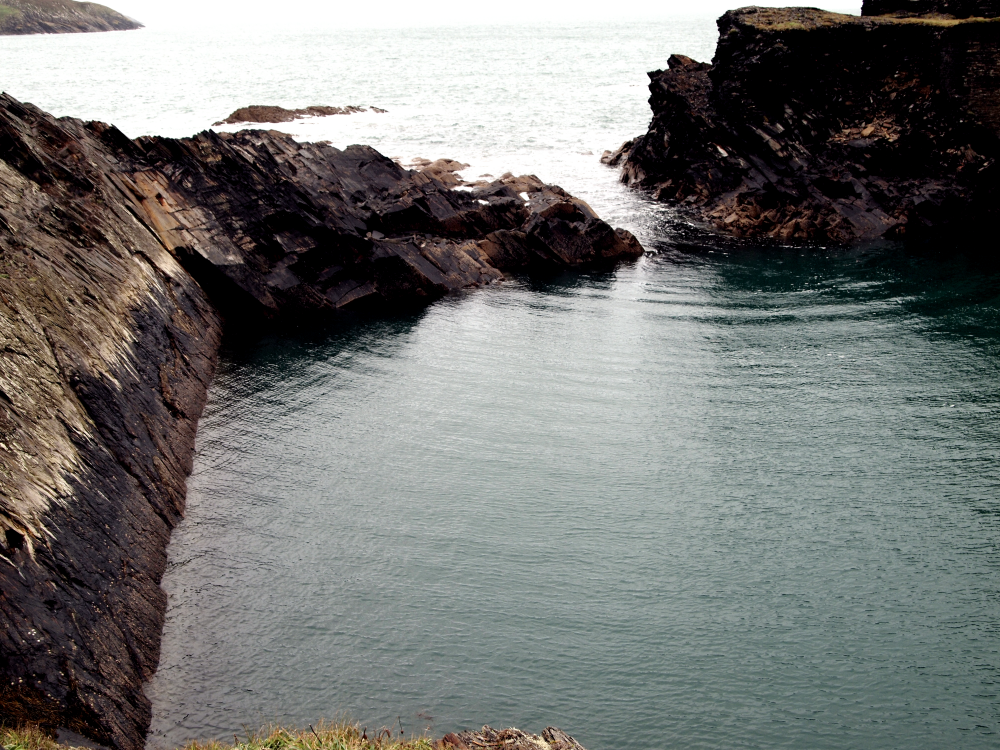
\includegraphics[width=0.9\linewidth]{images/beugung_von_wasserwellen.png}
\end{frame}

\begin{frame}{Grundlagen - Prinzip von Huygens}
    \includegraphics[width=\linewidth]{../../SeminarHarmonischeAnalysis/buch/papers/opt/images/huygens.pdf}
\end{frame}

\begin{frame}{Grundlagen - Beugung beim JWST}
    \begin{columns}
        \begin{column}{0.5\textwidth}
            \centering
            \includegraphics[width=\textwidth, page = 1]{../../SeminarHarmonischeAnalysis/buch/papers/opt/images/jwst_sechseck.pdf}
            Beugung am Spiegel
        \end{column}
        \pause
        \begin{column}{0.5\textwidth}
            \centering
            \includegraphics[width=\textwidth, page = 2]{../../SeminarHarmonischeAnalysis/buch/papers/opt/images/jwst_sechseck.pdf}
            Beugung an den Streben
        \end{column}
    \end{columns}
\end{frame}

\begin{frame}[plain]
    \begin{tikzpicture}[overlay, remember picture]
        \node[inner sep=0pt] at (current page.center)
        {\includegraphics[height=\pdfpageheight]{../../SeminarHarmonischeAnalysis/buch/papers/opt/images/jamesWebb_publicDomain.png}};
    \end{tikzpicture}
\end{frame}

\begin{frame}{Grundlagen - Wellendarstellung}
    \begin{columns}
        \begin{column}{0.5\textwidth}
            \begin{center}
                \includegraphics[width=\linewidth]{../../SeminarHarmonischeAnalysis/buch/papers/opt/images/welle.pdf}
            \end{center}
        \end{column}
        \begin{column}{0.5\textwidth}
            \begin{block}<1->{Welle aus Physik 3}
                \begin{align*}
                    \zeta(x, t)
                    &=
                    \zeta_0 \cdot \cos(\omega t - \vec{k}\cdot\vec{x})
                    \\
                    k
                    &=
                    \frac{\omega}{u}
                    =
                    \frac{2 \pi}{\lambda}
                \end{align*}
            \end{block}
            \begin{exampleblock}<2->{Komplexwertiger Zeiger}
                \begin{equation*}
                    \zeta(x, t)
                    =
                    \zeta_0 \cdot e^{j(\omega t - \vec{k}\cdot\vec{x})}      
                \end{equation*}
            \end{exampleblock}
        \end{column}
    \end{columns}
\end{frame}

\begin{frame}{Grundlagen - Maxwell}
    \begin{columns}
        \begin{column}{0.5\textwidth}
            \begin{center}
                \includegraphics[width=\linewidth]{../../SeminarHarmonischeAnalysis/buch/papers/opt/images/maxwell.pdf}
            \end{center}
        \end{column}

        \begin{column}{0.5\textwidth}
            \begin{block}{Erste Maxwellsche Gleichung}
                \begin{align*}
                    \oint_{S=\partial V} \varepsilon\vec{E} \cdot\, d\vec{S}
                    &=
                    \int_{V}\rho\, dV
                    \\
                \end{align*}
            \end{block}
            \pause
            \begin{block}{Angewandt}
                \begin{align*}
                    \int_{0}^{a}\int_{0}^{2\pi} \varepsilon E\cdot 1 \cdot r\, d\varphi dl
                    &=
                    Q
                    \\
                    2\pi ra\varepsilon E
                    &=
                    Q
                \end{align*}
            \end{block}
            \pause
            \begin{exampleblock}{Elektrische Feldstärke}
                \begin{equation*}
                    E(r)
                    =
                    \frac{Q}{2\pi\varepsilon a} \cdot \frac{1}{r}
                    =
                    C \cdot \frac{1}{r}
                \end{equation*}
            \end{exampleblock}
        \end{column}
    \end{columns}
\end{frame}

\begin{frame}{Grundlagen - Beugungsintegral}
    \begin{center}
        \includegraphics[width=0.7\linewidth]{../../SeminarHarmonischeAnalysis/buch/papers/opt/images/derivation.pdf}
    \end{center}
    \begin{block}{Geometrie gemäss Skizze}
        \begin{equation*}
            r
            =
            \sqrt{l^2 + (y_p-y)^2}
            =
            l \sqrt{1 + \frac{(y_p-y)^2}{l^2}}
        \end{equation*}
    \end{block}
    % \begin{equation*}
    %     E(y_p, t)
    %     =
    %     C\zeta_0 \cdot \int_{-\infty}^{\infty}f(y)\cdot\frac{e^{j(\omega t - \vec{k}\cdot\vec{r})}}{r} \,dy
    % \end{equation*}
    % \begin{equation}
    %     dE
    %     =
    %     E(r) \cdot \zeta(r, t) \cdot dy
    %     =
    %     \frac{C}{r} \cdot \zeta_0 \cdot e^{j(\omega t - \vec{k}\cdot\vec{r})} \cdot dy
    % \end{equation}
\end{frame}

\begin{frame}{Grundlagen - Beugungsintegral}
    \begin{columns}
        \begin{column}{0.5\textwidth}
            \centering
            \includegraphics[width=\linewidth]{../../SeminarHarmonischeAnalysis/buch/papers/opt/images/derivation.pdf}
        \end{column}

        \begin{column}<1->{0.5\textwidth}
            \begin{block}<1->{Geometrie gemäss Skizze}
                \begin{equation*}
                    r
                    =
                    \sqrt{l^2 + (y_p-y)^2}
                    =
                    l \sqrt{1 + \frac{(y_p-y)^2}{l^2}}
                \end{equation*}
            \end{block}
            \begin{block}<1->{Viele kleine Einflüsse}
                \begin{equation*}
                    dE
                    =
                    E(r) \cdot \zeta(r, t) \cdot dy
                    =
                    \frac{C}{r} \cdot \zeta_0 \cdot e^{j(\omega t - \vec{k}\cdot\vec{r})} \cdot dy
                \end{equation*}
            \end{block}
            \begin{block}<2->{Integriert über die Blende}
                \begin{align*}
                    E(y_p, t)
                    &=
                    \int_{y_b}^{y_b + b} E(r) \cdot \zeta(r, t) \cdot \,dy \\
                    &=
                    \int_{y_b}^{y_b+b}C\zeta_0 \cdot \frac{e^{j(\omega t - \vec{k}\cdot\vec{r})}}{r} \,dy
                    \end{align*}
            \end{block}      
        \end{column}
    \end{columns}
\end{frame}

\begin{frame}{Grundlagen - Beugungsintegral}
    \begin{block}<1->{Integriert über die Blende (cont.)}
        \begin{equation*}
            E(y_p, t)
            =
            C\zeta_0 \cdot \int_{y_b}^{y_b+b}\frac{e^{j(\omega t - \vec{k}\cdot\vec{r})}}{r} \,dy
            \end{equation*}
    \end{block}
    \begin{block}<2->{Blendenfunktion anstatt ein einzelner Spalt}
        \begin{equation*}
            f(y)
            \in
            [0, 1]
            \end{equation*}
    \end{block}
    \begin{exampleblock}<3->{Allgemeines Beugungsintegral}
        \begin{equation*}
            E(y_p, t)
            =
            C\zeta_0 \cdot \int_{-\infty}^{\infty}f(y)\cdot\frac{e^{j(\omega t - \vec{k}\cdot\vec{r})}}{r} \,dy
            .
            \end{equation*}
    \end{exampleblock}
    \strut \only<4->{\alert<4->{Nicht fundamental auflösbar} $\Longrightarrow$ Fresnel \& Fraunhofer Approximationen}  
\end{frame}
